%======================================================
%     H O W   T O   U S E   T H I S   F I L E
%  if you want to re-size the fonts in any of the columns, change the fontsize by un-hiding the NOTANONschedule tab in the Work Plan googlesheet,
%  then making the desired edits to the text in the yellow blocks, which are used to construct the latex code.
% A fontsize-selection menu is on that page for quick editing of fontsizes alone, but for color and other format changes,
% you will need to find the specific area on that sheet to edit
% .... also ...
% (1) download or connect to https://github.com/pmarcum/LaTex-Formatting and select the
%        set of files (aas-style or general) that meet your situation, you can either download the files or link
%        Overleaf to the needed files in the GitHub repository through URL, and then add the following to
%        the preamble of your main paper
%\usepackage{FUpackages}
%\usepackage{FUformatting}
%\usepackage{FUnewCommands} % not needed by WorPT files but generally useful
% (2) type the following into the main latex file where you want to put this table:
%\addtocounter{table}{-1} %corrects double-counting of sidewaystable and longtable combination
%\begin{sidewaystable}  %comment out if not needed
%   \begingroup
%      \setlength{\tabcolsep}{1pt}  % changes horizontal spacing between columns
%      \renewcommand{\arraystretch}{0.8} %changes vertical space between rows
%      \centerline{
%         \begin{minipage}{1.5\textwidth}  %wide table needs some of the margin?  change 1.5 to whatever
%            \begin{longtable} {|>{\raggedright\arraybackslash}p{4.1in} % title column
%
%               |>{\raggedright\arraybackslash}p{24ex}%task assignments (ID and \#Weeks)
%               |p{5ex}!{\color{lightgray}\vrule}p{5ex}!{\color{lightgray}\vrule}c|%TOTAL FTE columns
%               }
%               \expinput{do_NOT_manually_edit/NOTANONschedule}
%            \end{longtable}
%         \end{minipage}
%      }
%   \endgroup
%   \caption{\label{tab:NOTANONschedule} Resource-loaded project schedule, where: {\raisebox{-0.3\normalbaselineskip}[0pt][0pt]{
\begin{tikzpicture} \draw[fill=white,draw=red,line width=0.4mm] (0,0) circle[radius=0.2]; \draw[line width=0.4mm,red] node[midway,black]{\faDollar} (0.15,0.15) -- (-0.15,-0.15);  \draw[line width=0.4mm,red] (0.15,0.15) -- (-0.15,-0.15);  \end{tikzpicture}}} Not funded by this grant,  {\raisebox{-0.3\normalbaselineskip}[0pt][0pt]{\begin{tikzpicture}  \draw[fill=green,draw=black] (0,0) circle[radius=0.2];  \draw[draw=green] (-0.015,0.015) -- (0.015,-0.015) node[midway]{\faDollar};  \end{tikzpicture}}} funded by this grant, {\textbf{\large{$\Sigma$}}} funded $+$ unfunded; Tasks are listed (left side), with duration of task activity indicated in blue-colored timelines  that measure quarter-years (1,2,3,4). Task assignments identify specific team members responsible for  implementation with associated work weeks, where color indicates institutional affiliation  (blue$=$funded/U.S., black$=$not funded/U.S., red=international). "Total FTE" (right side) are integrated work-weeks converted into FTE per task (1~FTE$=$12~months), displayed as "total",  "unfunded by this grant", and "funded by this grant", resp.  Asignment identities:  {\textbf{dd}}: Dan.Dent{\'{o}}n, {\textbf{pm}}: Pamela.Marcum, {\textbf{ss}}: Sally.Smith}
%\end{sidewaystable}  % comment out if not used
%======================================================
%
% ----------------------- First / top line of headers
\multicolumn{1}{c|}{} % title column
&
& \multicolumn{1}{c}{} %task assignment column
& \multicolumn{3}{c}{}\\ % 3-column total fte
%
% ------------------------- Second line of headers
\multicolumn{1}{c|}{} % title column
%
& \multicolumn{1}{c|}{\scriptsize{TASK}} %task assignments column
& \multicolumn{3}{c|}{\scriptsize{TOTAL}}\\ % 3-column total fte
%
% -------------------------  Third line of headers
\multicolumn{1}{c|}{} %title column
%
& \multicolumn{1}{c|}{\scriptsize{ASSIGNMENTS}} %task assignments in ID and \#week pairs
& \multicolumn{3}{c|}{\scriptsize{FTE}}\\ % 3-column total fte
\cline{1-1}
% -------------------------  Forth line of headers
\multicolumn{1}{|l|}{\normalsize{TASK TITLES}} % title column
& \scriptsize{1} & \scriptsize{2} & \scriptsize{3} & \scriptsize{4} %Yr1
%
%
%
%
& \multicolumn{1}{c|}{\scriptsize{id~\#wks}} %task assignments in ID and \#week pairs
& {\textbf{\large{$\Sigma$}}} % Col1 Total FTE
& {\raisebox{-0.3\normalbaselineskip}[0pt][0pt]{
\begin{tikzpicture}
\draw[fill=white,draw=red,line width=0.4mm] (0,0) circle[radius=0.2];
\draw[line width=0.4mm,red] node[midway,black]{\faDollar} (0.15,0.15) -- (-0.15,-0.15);
\draw[line width=0.4mm,red] (0.15,0.15) -- (-0.15,-0.15);
\end{tikzpicture}}} % Col2 Total FTE
& {\raisebox{-0.3\normalbaselineskip}[0pt][0pt]{\begin{tikzpicture}
\draw[fill=green,draw=black] (0,0) circle[radius=0.2];
\draw[draw=green] (-0.015,0.015) -- (0.015,-0.015) node[midway]{\faDollar};
\end{tikzpicture}}}% Col3 Total FTE
\hline
%beginning level 1 task
{\normalsize\textbf\scshape{A}}~{\normalsize\textbf{Data and models preparation}}
& {} % mpty year quarters
&{} %empty task assignments
&\tiny{}&\tiny{}&\tiny{}\\ %empty total FTEs
%beginning level 2 task
~{\scriptsize{\textbf{\scshape{A1}}}}~{\color{mediumelectricblue}{\footnotesize\textbf{Generate simulated data}}}
&{\tiny\cellcolor{mediumelectricblue}}&{\tiny\cellcolor{mediumelectricblue}}&{\tiny}&{\tiny}&{\tiny}&{\tiny}&{\tiny}&{\tiny}&{\tiny}&{\tiny}&{\tiny}&{\tiny}
&{ss\,8 {\small\color{blue}pm}\,{\small\color{blue}2} {\small\color{blue}dd}\,{\small\color{blue}4}}
&{\small0.27}&{\small0.04}&{\small\color{blue}0.23}\\
%beginning level 2 task
~{\scriptsize{\textbf{\scshape{A2}}}}~{\color{mediumelectricblue}{\footnotesize\textbf{Make emission maps}}}
&{\tiny\cellcolor{mediumelectricblue}}&{\tiny\cellcolor{mediumelectricblue}}&{\tiny\cellcolor{mediumelectricblue}}&{\tiny}&{\tiny}&{\tiny}&{\tiny}&{\tiny}&{\tiny}&{\tiny}&{\tiny}&{\tiny}
&{{\small\color{blue}dd}\,{\small\color{blue}6} {\small\color{blue}ss}\,{\small\color{blue}6}}
&{\small0.23}&{\small0.00}&{\small\color{blue}0.23}\\
%beginning level 2 task
~{\scriptsize{\textbf{\scshape{A3}}}}~{\color{mediumelectricblue}{\footnotesize\textbf{Incorporate thermal emission models}}}
&{\tiny}&{\tiny}&{\tiny\cellcolor{mediumelectricblue}}&{\tiny}&{\tiny}&{\tiny}&{\tiny}&{\tiny}&{\tiny}&{\tiny}&{\tiny}&{\tiny}
&{{\small\color{blue}ss}\,{\small\color{blue}6} {\small\color{black}pm}\,{\small\color{black}4}}
&{\small0.19}&{\small0.08}&{\small\color{blue}0.12}\\
\hline
%beginning level 1 task
{\normalsize\textbf\scshape{B}}~{\normalsize\textbf{Application to archive}}
& {} % mpty year quarters
&{} %empty task assignments
&\tiny{}&\tiny{}&\tiny{}\\ %empty total FTEs
%beginning level 2 task
~{\scriptsize{\textbf{\scshape{B1}}}}~{\color{mediumelectricblue}{\footnotesize\textbf{Determine fields of interest}}}
&{\tiny}&{\tiny}&{\tiny\cellcolor{mediumelectricblue}}&{\tiny\cellcolor{mediumelectricblue}}&{\tiny\cellcolor{mediumelectricblue}}&{\tiny}&{\tiny}&{\tiny}&{\tiny}&{\tiny}&{\tiny}&{\tiny}
&{pm\,4 {\small\color{blue}dd}\,{\small\color{blue}2} {\small\color{blue}ss}\,{\small\color{blue}2}}
&{\small0.15}&{\small0.04}&{\small\color{blue}0.12}\\
%beginning level 2 task
~{\scriptsize{\textbf{\scshape{B2}}}}~{\color{mediumelectricblue}{\footnotesize\textbf{Reduction of image mosaics}}}
&{\tiny}&{\tiny}&{\tiny}&{\tiny}&{\tiny\cellcolor{mediumelectricblue}}&{\tiny\cellcolor{mediumelectricblue}}&{\tiny\cellcolor{mediumelectricblue}}&{\tiny}&{\tiny}&{\tiny}&{\tiny}&{\tiny}
&{{\small\color{blue}dd}\,{\small\color{blue}10} {\small\color{blue}ss}\,{\small\color{blue}4}}
&{\small0.27}&{\small0.00}&{\small\color{blue}0.27}\\
\hline
%beginning level 1 task
{\normalsize\textbf\scshape{C}}~{\normalsize\textbf{Documentation and publications}}
& {} % mpty year quarters
&{} %empty task assignments
&\tiny{}&\tiny{}&\tiny{}\\ %empty total FTEs
%beginning level 2 task
~{\scriptsize{\textbf{\scshape{C1}}}}~{\color{mediumelectricblue}{\footnotesize\textbf{Code documentation and user system verification}}}
&{\tiny}&{\tiny}&{\tiny}&{\tiny}&{\tiny}&{\tiny\cellcolor{mediumelectricblue}}&{\tiny\cellcolor{mediumelectricblue}}&{\tiny\cellcolor{mediumelectricblue}}&{\tiny\cellcolor{mediumelectricblue}}&{\tiny}&{\tiny}&{\tiny}
&{{\small\color{blue}ss}\,{\small\color{blue}8} {\small\color{blue}dd}\,{\small\color{blue}3} {\small\color{black}pm}\,{\small\color{black}6}}
&{\small0.33}&{\small0.12}&{\small\color{blue}0.21}\\
%beginning level 2 task
~{\scriptsize{\textbf{\scshape{C2}}}}~{\color{mediumelectricblue}{\footnotesize\textbf{Pub 1: pipeline and improved images}}}
&{\tiny}&{\tiny}&{\tiny}&{\tiny}&{\tiny}&{\tiny}&{\tiny}&{\tiny\cellcolor{mediumelectricblue}}&{\tiny\cellcolor{mediumelectricblue}}&{\tiny\cellcolor{mediumelectricblue}}&{\tiny}&{\tiny}
&{{\small\color{blue}dd}\,{\small\color{blue}8} {\small\color{blue}pm}\,{\small\color{blue}2} {\small\color{blue}ss}\,{\small\color{blue}6}}
&{\small0.31}&{\small0.00}&{\small\color{blue}0.31}\\
%beginning level 2 task
~{\scriptsize{\textbf{\scshape{C3}}}}~{\color{mediumelectricblue}{\footnotesize\textbf{Pub 2: galaxy identification}}}
&{\tiny}&{\tiny}&{\tiny}&{\tiny}&{\tiny}&{\tiny}&{\tiny}&{\tiny}&{\tiny\cellcolor{mediumelectricblue}}&{\tiny\cellcolor{mediumelectricblue}}&{\tiny\cellcolor{mediumelectricblue}}&{\tiny\cellcolor{mediumelectricblue}}
&{{\small\color{blue}pm}\,{\small\color{blue}8} {\small\color{blue}dd}\,{\small\color{blue}4} {\small\color{blue}ss}\,{\small\color{blue}4}}
&{\small0.31}&{\small0.00}&{\small\color{blue}0.31}\\
\hline